\chapter{Quality-Centric Data Model}
\label{ch:data_model}

Overload in a stream processing system has been usually considered as a transient and rare condition. The
common approach to handle overload has been to recover from it as quickly as possible, without
quantifying its impact on the current processing. In many large-scale deployments, however, the
occurrence of overload is common and not always avoidable. In such cases, it is better to adapt the
system so that it can self-inspect and quantify the impact of overload on the computed results and let
the user decide if the quality of the output is acceptable or not. 

In order to do so, the system should quantify the amount of information that was lost during the
processing because of failure. A quality metric can be used to enhance streams and detect and
estimate the impact of failure on the current computation. Such a metric should be generic enough so
that it can be used in any stream processing system, supporting the semantics of traditional as well as
custom operators, and be applicable to a broad variety of query types.
 
This chapter presents the quality-centric data model that we have
developed to allow a stream processing system to calculate the impact of failure on its running queries.
First, we provide a set of definitions about the basic components of a stream processing
system, as they are assumed in the scope of this work. These fundamental concepts are used then to
describe the workings of a stream processing system and to define a suitable quality metric.

In order to define such a metric, it is important to understand the goals and the assumptions.
We provide an explanation about the reasoning behind such a metric and about the characteristics
that it should have. Next, we introduce the two main families of queries, fan-in and
fan-out, providing sample queries to illustrate them.

We then introduce the Source Information Content (\sic) metric, a quality metric
defined based on the previous assumptions and with the required characteristics. A set of equations are
given for its calculation, describing its propagation within the system and the benefits of its use.

The chapter closes with running examples of real queries taking advantage of the \sic metric to
enhance their processing so that failure can be detected and accounted for automatically. They show
how the \sic metric can be applied to different query types and how its behaviour directly derives from
the previously stated assumptions.

\section{Model Definitions}
\label{sec:definitions}
This section presents the definition of the basic components of a stream processing system as
they are used in this work. Many of the concepts are similar or equivalent to their
counterparts already described when presenting the CQL and boxes-and-arrows query models in
Section~\ref{sec:querymod}.
Nevertheless, a precise definition of many concepts used throughout this thesis is necessary for the correct
understanding of this work. Table~\ref{tab:notation} summarises the notation used below.
%--------------------------------------------------------------------------------------------------------
\subsection*{Schema}
In order for the system to be able to interpret the content of a unit of information, it is necessary to
describe the values that it contains, providing a name and a data type for each item. 
Such a definition is contained in a \emph{schema}.
\begin{definition}[Schema]{ 
A schema $S$ is a data structure of elements in the form: $\langle Type, Name \rangle$.}
\end{definition}
A \textit{schema} defines the structure of the payload contained in a tuple. It is formed by a series
of $\langle Type, Name \rangle$ pairs, each specifying the abstract type and the name of an item. It
is equivalent to a schema used in a relational database, where it is used to describe the columns forming a
table. 

\underline{\textsc{Example}}: Consider a tuple with the following schema:\\

\begin{table}[th!]
	\centering
	\begin{tabular}{|c||c|} \hline
	%notation & description \\ \hline
	\textit{Integer} 	&	\textsc{NodeID}		\\	\hline
	\textit{Double}		&	\textsc{CpuLoad}	\\	\hline
	\textit{Long}		&	\textsc{UpTime}		\\	\hline
	\end{tabular}
	
	%\caption{Schema of a tuple containing load and uptime information for a specific processing node.}
	\label{table:schema}
\end{table}

It contains information about load and uptime for a specific sensor. Each field has a name so that
it can be referred to when processing the tuple and it includes an abstract type, which will be
translated to a system type once the tuple is instantiated.\\

%--------------------------------------------------------------------------------------------------------
\subsection*{Tuple}
A schema describes the prototype for a data item processed by a stream processing system. 
An instance of a schema containing actual information to be processed is called a \emph{tuple.}

\begin{table}[t!]
\centering
\begin{tabular}{|c||c|} \hline
%notation & description \\ \hline
\multicolumn{2}{|c|}{{\bf Model Notation}} \\ \hline \hline
$t$                     & tuple\\ \hline
%$t_{\tau}$             & generation timestamp of tuple $t$  \\ \hline
$\tau$	           		& tuple timestamp  \\ \hline
%$t_{SIC}$               & \qm value of tuple $t$ \\ \hline
$QM$               		& tuple quality metric value \\ \hline
%$t_{\mathcal{V}}$       & set of schema values of tuple $t$ \\ \hline
$\mathcal{V}$       	& tuple payload \\ \hline
$S$						& abstract stream of tuples \\ \hline
$B$						& batch of tuples \\ \hline
$O$         		    & operator \\ \hline
$f_{op}$                  & operator function \\ \hline
$Q$			            & query \\ \hline
$f_{Q}$                  & query function \\ \hline
$\mathcal{S}$          & set of all sources attached to a query \\ \hline
$\mathcal{T}^{S}$      & source information tuple set  \\ \hline
% %$\mathbb{T}^{S}$       & set of source tuples space \\ \hline
% $*t^{R}$                 & query result tuple  \\ \hline
% $*\mathbb{T}^{R}$        & stream of query result tuples \\ \hline
% $*f$                     & query function \\ \hline
% $*f^{-1}$                & inverse query function \\ \hline
% $*\mathcal{T}_{in}^{o}$  & set of input tuples to operator $o$  \\ \hline
% $*\mathcal{T}_{out}^{o}$ & set of output tuples of operator $o$  \\ \hline
% %\multicolumn{2}{|c|}{{\bf notation for the data streaming system}} \\ \hline \hline
% $*\mathcal{N}$           & set of nodes \\ \hline
% $*\mathcal{Q}$           & set of queries \\ \hline
% $*\mathbb{T}^{R}_{q}$    & stream of result tuples for query $q$\\ \hline
\end{tabular}
\caption{Notation used in the model definitions.\label{table:query}}
\label{tab:notation}
\end{table} % TABLE DEFINITIONS

\begin{definition}[Tuple]{ 
A tuple is an element $t = \langle \tau, QM, \mathcal{V} \rangle$ where $\tau \in T$ is the
timestamp of the element, QM is a quality metric metadata value and 
$\mathcal{V}$ is a set of values defined by a schema $S$.
}
\end{definition}

A \textit{tuple} is the basic information vector in a stream processing system, representing a
single unit of data. In our model, a tuple is composed by three main elements: a
\textit{timestamp}, a \textit{quality metric} and a \textit{payload}.

With timestamp ($\tau$) we mean an temporal indication of when the tuple was produced. This typically is
the time at which the tuple entered the system. In this case, the sources are only concerned with the
production of the raw data and timestamps are assigned by the system as the UTC time at the moment of
input. It is also possible for the timestamp to be set externally, which is useful in case
of synthetic workloads. In this case, the timestamp is determined by an external entity.

In our model, a tuple is always augmented with a \emph{quality} metadata value ($QM$), which is an
indication of the amount of information that is contained in the tuple. This value is maintained by the
system and varies according to the amount of failure (\ie tuple loss) that occurred during the
processing of the tuple.
It has two main functions: it reports back to the user the achieved quality of processing for the
current processing, and it is used internally by the system to make intelligent load-shedding decisions
under overload.

The third element composing a tuple is the \textit{payload} ($\mathcal{V}$). It contains the actual
information carried by the tuple. It is formed by one or more values of any primitive data type. 
The type and the order of the values forming a tuple payload is defined by the schema.

Logically, we can divide tuples in three categories: a \textit{source} tuple ($t_{src}$) is a tuple
generated from a data source representing a single input to the system; a \textit{derived} tuple ($t_{op}
\in \mathcal{T}_{out}^{o}$) is a tuple generated by an intermediate operator; and, finally, there exist
\textit{result} tuples ($t_{res}$), which are derived tuples produced by a terminal operator. They
contains the final results of the processing, which are delivered to the user together with the \qm
value.

\underline{\textsc{Example}}: Figure~\ref{fig:tuple} shows a simple tuple with its relational schema.
It shows a \emph{timestamp} expressed as POSIX time, a \emph{quality metric} value and a \emph{payload}
with three fields carrying information about the CPU load and uptime of a machine monitored by the system.
We discuss the implementation of tuples in Section~\ref{sec:tuples}.
\begin{figure}[t]
	\centering
	\includegraphics[width=0.8\textwidth]{img/tesi/tuple}
	\caption{A simple tuple with the relational schema.}
	\label{fig:tuple}
\end{figure}
%--------------------------------------------------------------------------------------------------------
\vspace{-10pt}
\subsection*{Stream}
A \emph{stream} is an abstract entity that describes all tuples flowing between two
operators. The number of tuples is potentially infinite and all tuples share a common schema.
\begin{definition}[Stream] {
A stream is a potentially unbounded time-ordered sequence of tuples, all belonging to the same schema.}
\end{definition}
A \textit{stream} is a logical abstraction, representing the totality of the
tuples flowing between two operators. It is time ordered, meaning that a tuple $t_2$ received after a
tuple $t_1$ always has a timestamp greater than or equal to $t_2$ (\ie $\tau_2 \geq \tau_1$).

% We can distinguish between  streams, \textit{derived} streams and \textit{output} streams.
Analogous to tuples, streams can be divided into three categories: \textit{base} streams ($S_{src}$) are
generated from sources and are the input to the system; \emph{derived} streams ($S^{o}_{out}$) are
produced as an output by the operators of a running query; and \emph{result} streams ($S_{res}$) are
derived streams produced by a terminal operator, which contain the results of the processing delivered
to the user.

A stream is used only logically to describe a potentially unbounded sequence of tuples flowing between
two operators. The system, however, needs a finite amount of tuples to operate, which in our system is
represented by a \textit{batch}.

%--------------------------------------------------------------------------------------------------------
\subsection*{Batch}
Streams are continuous abstract entities, while operators need a finite set of tuples to operate.
The system thus partitions streams into \emph{batches}: finite snapshots of a stream, containing
tuples that have the same \emph{quality metric} value to be used as input and output units for
operators.

\begin{definition}[Batch]{
A batch is a finite set of tuples $B=\{t_1,\dots,t_n\}$, all having the same \qm metadata value.
}
\end{definition}

A \textit{batch} is a logical group of tuples with the same quality metric value. In our model, an
operator does not work on a single tuple but on batches. It processes one or more input batches and produces one
output batch, which may be composed of a single tuple.
Using batches allows for a more compact representation of the \qm metadata because it does not have to be
included with each tuple. It also speeds up the calculation of the new \qm value when an operator
outputs a new set of tuples.
 
Batches represent a snapshot of a stream (\ie a finite amount of tuples that can be processed by an
operator). In our system, they are the equivalent to \textit{relations} used in CQL.
The discussion about our implementation of batches is given in Section~\ref{sec:batches}.

%--------------------------------------------------------------------------------------------------------
\vspace{-10pt}
\subsection*{Operator}
A stream processing system transforms a set of input tuples into a set of output tuples representing the
answer to a given query. This data transformation used to produce a result is carried out by a number
of \emph{operators}.


\begin{definition}[Operator]{
An operator is a function $f_{op}$ over a set of input streams $S_{in}=\{S_1,\dots,S_n\}$,
that generates a new output stream $S_{out}$=$f_{op}(S_{in})$. 
}
\end{definition}
 
An \textit{operator} is the basic processing unit in a stream processing system. It represents a
function over a set of input streams, transforming  one or more input batches into one output batch. 

Operators are seen as \textit{black boxes} in our system, meaning that their internal semantic is not
taken into account when calculating the \qm value for the newly generated derived tuples.
We can divide operators based on their behaviour when handling input streams into two categories:
\textit{blocking} or \textit{non-blocking} operators.

Blocking operators need to have at least one input batch available on each of their input
streams. For example, if there are two inputs to an operator, one containing two input
batches while the other one is currently empty, the operator blocks until an input batch arrives
on the second input stream. When this happens, the first batch of each input is removed and processed,
producing one derived batch. Assuming no other batch has arrived on the second input, the operator
blocks again, as only the first input contains data to be processed.

Non-Blocking operators do not need input on all channels to be triggered. Instead, they produce
a derived batch as soon as at least one input batch is present on one of their input channels. 
Such an operator never blocks waiting for input and never has pending input data.
%The discussion about our implementation of queries is given in Section~\ref{sec:queries}.

\begin{figure}[b!]
	\centering
	\includegraphics[width=0.7\textwidth]{img/tesi/operator} 
	\caption{A black-box operator with two input and one output stream.}
	\label{fig:tuple}
\end{figure}

%--------------------------------------------------------------------------------------------------------
\vspace{-10pt}
\subsection*{Query}
The processing required to transform the information contained in input tuples into a useful
output for the user is typically not performed by a single operator but by a group of them, arranged into
a logical processing graph. This graph is referred to as a \emph{query}.

 \begin{definition}[Query]{
A query logically defines a series of processing steps over a set of input streams 
$S_{in}=\{S_{in}^1,\dots,S_{in}^n\}$ to produce a desired set of output streams 
$S_{out}=\{S_{out}^1,\dots,S_{out}^n\}$ by the means of a finite number of operators.
}
\end{definition}
%%\mnote{Does it need better definition? How?}

A query describes the processing to transform a set of input streams into a set of output streams.
In the boxes-and-arrows model, queries are depicted as a directed acyclic graph (DAG), in which arcs
represent streams and vertices represent operators. One or more sources produce streams of tuples at
time-varying rates, which are the input to the system. One or more operators process these
tuples, either in sequence or in parallel.

A query is a graph, in which vertices correspond to operators and arcs indicate the direction of tuples
flowing from one or more sources to one or more terminal operators. The set of query operators is
given by $\mathcal{O}$ and cumulatively computes the query function $f_Q$. Operators may be distributed
over a set of nodes $N$ if the query function is too complex to be computed on a single machine.
The discussion about our implementation of queries is given in Section~\ref{sec:queries}.

%--------------------------------------------------------------------------------------------------------


\begin{comment}
\section{Quality-Centric Data Model}
\todo{Rewrite Introduction}
In this section I will start presenting the \textit{quality-centric data model} we have developed, with
the aim of increasing the system \textit{dependability} and to reason about the achieved
\textit{quality-of-service}.
I will first describe a novel metric called \textit{Source \DIFdelbegin \DIFdel{Information Content}\DIFdelend \DIFaddbegin \DIFadd{Coverage Ratio}\DIFaddend } (\sic), which is a
metadata value associated with data streams. Then I will provide some foundation assumptions we made in
the design of it and the reasoning behind these decisions.
\end{comment}

\begin{comment}
\DIFdelbegin %DIFDELCMD < \subsection***{Source Information Content}
%DIFDELCMD < %%%
\DIFdelend \DIFaddbegin \subsection***{Source Coverage Ratio}
\DIFaddend 

In a traditional stream processing system streams only contain data associated with
timestamps, they do not carry information about the failure experienced by the system. In our model we
propose to augment streams so that failure is recorded and accounted for. In order to do so we introduce
a new metric called \textit{Source \DIFdelbegin \DIFdel{Information Content}\DIFdelend \DIFaddbegin \DIFadd{Coverage Ratio}\DIFaddend } (\sic) that gives a hint about the amount of
information contained in a tuple and thus to its importance for the current query results. This is added
to streams in the form metadata, whose value is calculated by the query operators and is inversly
proportional to the occurrence of failure.

A tuple should convey information about the amount of failure experienced during its creation. There
should be a way to indicate if the data carried by a tuple was created using all the available
information, and is then 100\% accurate, or if some information was lost in the process, thus reducing
the dependability of that data. \textit{Source \DIFdelbegin \DIFdel{Information Content}\DIFdelend \DIFaddbegin \DIFadd{Coverage Ratio}\DIFaddend } tries to do achieve
this goal, by measuring the amount of lost information in the creation of a tuple.

The system can use this value to make decision about the importance of a tuple towards the creation of
the final query result. When the system is overloaded for instance, it has to decide which tuples should
be dropped in order to recover. \sic values in this case can be used to assess the individual value of
tuples and guide the system to a selection that helps improving the quality of the results.

In a single query scenario the system is able to reason about the amount of information carried by
tuples, by dropping the ones with the lowest values it minimises the impact on the query results. Even in
the absence of failure it may be that some tuples aggregate more information than others and should be
treated with more care. In case of failure then, the system would prefer to drop some already compromised
tuples before other which where produced with perfect information.

When dealing with a system that allows the the concurrent execution of multiple queries, \sic values
help discarding tuples so that all queries in the system are affected in the same way. All qu
This process is referred to as  \textit{fair shedding} and will be further analysed in
Section~\ref{sec:fair shedding}.

In the next section I will present some assumption we made about the \sic quality metric, giving some
reasoning behind them. I will not introduce any formulas at this point, leaving the discussion about how
\sic values are c alculated to Section~\ref{sec:sic}.
\\
\end{comment}

\section{Model Assumptions}
\label{sec:assumptions}

% In the design of a suitable quality metric that could be used to capture the amount of failure
% occurring in the processing of a query, there need to be some assumptions that limit and define it.
This section states the assumptions that led to the definition of a quality metric called Source
Information Content (\sic), which is presented formally in Section~\ref{sec:sic}.
It is based on the consideration that overload is a common condition and should not be ignored but
accounted for. Instead of trying to mask it, the system should monitor it and report its impact.
Since queries can be composed of an arbitrary set of operators, frequently employing diverse processing
semantics, a quality metric must be sufficiently generic to be usable across the whole spectrum of
possible queries and not tied to a specific domain. \\
When considering data sources, it is possible that some of the produced inputs are more valuable than
others but it is often difficult to decide this beforehand. The challenge of determining which sources
and tuples are more valuable than others leads to the idea of considering all tuples as equally
important. When an operator receives some tuples as input, it transforms them but does not change the
amount of information that they carry.
Conceptually, this is similar to the conservation of energy law in physics.
Another consideration is that the amount of information in a tuple is proportional to the amount of
tuples required for its generation. Since we assume that every source produces the same amount of
information per time interval, the total amount of information processed by a query in the absence of
failure is a multiple of the number of sources. Finally, we consider the shape of a query graph, which,
in its most generic form, is a directed acyclic graph. The computation of the quality metric should be
flexible enough to be usable for all graphs. \\
The rest of the section describes these assumptions in more detail, laying out the reasoning that lead to
the Source \DIFdelbegin \DIFdel{Information Content }\DIFdelend \DIFaddbegin \DIFadd{Coverage Ratio }\DIFaddend (\sic) quality metric.\\

\textbf{1. FAILURE IS EVERYWHERE\\ \textit{Failure is always present in large-scale query processing,
and overload is a kind of failure.}}

  In large-scale distributed systems, failure cannot be considered a rare and transient condition.
  In fact, evidence suggests that, in such systems, a certain percentage of nodes will be failing at
  all times. Even though the Mean Time Between Failure (MTBF) for a single component may be quite high,
  once the number of components increases, failures become more and more relevant. 

  In a paper released by Google~\cite{google-failure-disks}, it is shown how the occurrence of failure in
  a large hard disk population is higher than what is declared by vendors. They analyse a large
  population of disks and showed how the Annualized Failure Rate (AFR) ranges from 1.7\% for first-year
  drives to over 8.6\% for three-year old drives.
  Jeff Dean of Google also presents statistics~\cite{google-failure-talk} about the real world occurrence
  of failure in their data centres, showing that a typical cluster of 2400 machines it is expected to
  experience around 1000 individual machines failures in the first year alone. 
%   There is a 50\% chance that a cluster overheats, taking down most of the servers in less than 5 minutes
%   and taking 1 to 2 days to recover.
%   
  Overload can be considered as a type of failure because the system cannot process all the
  incoming data and must discard some of it. In this case, an approximate result is produced even
  though all the processing units function correctly.
  Input data rates can be highly unpredictable, with variations that can often be of orders of
  magnitude~\cite{load-shedding}. This makes it challenging to provision a system. 
  If we consider a cloud deployment scenario, in which resources are rented, overload can not
  only be tolerated but may be deliberate. It may be cheaper to underprovision the system on purpose in
  order to keep the costs down when the approximation of results is not an issue.  
  In case of a federated resource pool, in which several parties share their local clusters to gain access
  to a unified processing infrastructure, the possibilities for overload are even higher. Each local
  site, in fact, is under the control of a different authority, making recovery
  times unpredictable. Due to its nature as a shared platform, the processing resources available at each
  cluster are not uniform. The query fragments distributed across several processing sites thus
  experience a skewed availability of resources. For example, the same query fragment may run without failure at one
  site, while experiencing heavy overload at another.\\

\textbf{2. APPROXIMATE PROCESSING \\ \textit{Users can accept approximate processing but they need to have a
way of evaluating the quality of the computed results.}}

 	Failure should be considered a normal condition of operation for a large data stream processing
	system. We propose to augment data streams with a metric that captures the amount of failure during
	the processing. This quantifies the impact of failure instead of hiding it. 
	In many applications, an approximate result is acceptable for users. It is up to the user to decide if the quality
	of the delivered results is good enough for these to be accepted or if they should be discarded.

In sensor networks, it is common to have a lot of failure at the data source level. Sensors can suddenly
stop working because of hardware failure or can become temporarily unreachable. In such cases, a query
that processes sensor readings delivers results that are incomplete. Nevertheless, the quality of the
query results can be sufficient to be meaningful to the user. Especially when dealing with a large set of
sensors, the lack of input from a certain number of them does not mean that the computation should be
discarded altogether. Instead, the results become less accurate due to the missing input data. If we
consider queries aggregating readings for sensors scattered over a geographic area, such as an average of
measured pollutants in a city, it is possible that a failed sensor is located close to others that
record an equivalent reading. Thus the missing information may not produce a significant variation in the final
result, which is approximate yet still meaningful.

If we consider queries that detect a certain event instead, the failure of a single sensor can become
critical. The failed sensor could be the one that would have generated a reading of interest but, due to
the failure, this reading is not available. In this scenario, failure reduces a user's confidence in the
results and may not be tolerable. Even if an approximation of the results may not be acceptable, it is
important to notify the user that some failure occurred during the collection of the input data, leaving
the final decision about the confidence in the results to the user.

An analogous argument can be made for the social media analysis scenario. In this case, the enormous
amount of available input data can cause an overload condition of the processing infrastructure.
Unlike the sensor data scenario, in which the failure usually occurs at the input level, the failure here
is more likely to happen at the processing stage. Aggregation queries typically process vast amounts of
data and, in case of the loss of a small percentage of data, they can still produce results close to what
would have been obtained in the absence of failure. In general, when dealing with aggregation, the larger
the set of input data, the more tolerable failure becomes.\\

\textbf{3. A GENERIC QUALITY METRIC \\ A quality metric should be operator independent, abstracting
the query semantics.}

Stream processing systems are versatile and can compute a variety of queries. Each query is composed of
operators whose semantics can be different. If we consider the streaming equivalent of traditional
operators present in a relational DBMS, such as \textit{filter} and \textit{average}, it is notable how
the discarding of a tuple from the input of these operators can lead to significantly different quality
reductions in the produced output. Due to their different processing semantics, missing a single tuple
can have almost no influence or can completely alter the output of an operator.
Furthermore, it is common for stream processing systems to be extensible, allowing users to implement
their own custom operators, whose processing semantics are unknown a priori.

Let us consider the different impact that the loss of a tuple can have on operator results.
An average operator \DIFdelbegin \DIFdel{, }\DIFdelend that inputs a set of $100$ tuples with integer values uniformly distributed in the
range $[0,1]$, produces a single output tuple with a value close to $0.5$.
If we assume that $50\%$ of the input tuples are discarded due to overload, the operator still produces a
single tuple with a value close to $0.5$. In this scenario, the loss of half of the input tuples has
virtually no impact.

A filter operator with the same input tuples outputs only tuples with values below $0.5$. Since
the input is uniformly distributed, it produces on average an output of $50$ tuples.
When shedding half of the input values though, the operator result changes considerably. On average, it
now produces $25$ output tuples, which is half of the number of tuples that it would produce with the
complete set of input tuples. With this simple example, we can observe how the processing semantics of
the operator can be different: the impact of input loss can be almost unnoticeable for some operators
while it can be disruptive for others.

Therefore, the quality metric should be operator independent and valid for any kind of processing
semantics, efficiently capturing the processing degradation under failure. Even though the knowledge of
the internal functioning of operators would allow the system to have a more precise reasoning about the
impact of failure on the quality of the results, this is impractical for a general purpose system.
Instead of trying to quantify the approximation of the result in terms of  precision, we try to quantify
the amount of information that was lost during the computation of a result compared to the total amount
that would have been processed in the absence of failure.

Other \DIFdelbegin \DIFdel{proposal }\DIFdelend \DIFaddbegin \DIFadd{proposals }\DIFaddend for an operator independent approach exists. The \textit{network imprecision}  metric
accounts for the state of all participating nodes in a large-scale monitoring
system~\cite{network-imprecision}.
It estimates the percentage of nodes available when calculating an aggregate value over a set of data
sources. In contrast, our metric operates at the granularity of individual tuples, not sources, to reason
about the impact of information loss on the results.
Another example is the \textit{harvest} quality metric proposed by Murty and
Welsh~\cite{dependable-is-sensing} and Fox and Brewer~\cite{Fox1999}. The authors argue that harvest
should capture the fraction of data sources available in an Internet-scale sensor system. \\

\textbf{4. DATA SOURCE EQUALITY \\ \textit{All sources are equally important for the generation of the
final result data.}}

In our model, sources are all considered equally important, regardless of their tuple production rate.
If we consider a sensor network deployment, it is common to observe different rates of input readings.
This is due to different sensor settings or different battery constraints of the sensors. A unit with a
depleted battery may reduce the rate at which it propagates information to save energy.
Another reason could be the position of a sensor. The energy cost of propagating a reading grows with
distance because it requires a higher transmission power.

	Consider a sensor network monitoring humidity levels in a rural area, composed of sensors randomly
	scattered over a certain region. The processing query produces an average humidity value for the area
	every hour, aggregating readings from all sensors, which are produced once every $10$
	minutes. Due to the uneven distribution of sensors, some may require more power to transmit their
	readings and, in order to save battery power, may decide to reduce their transmission rate to half the original rate. 
	When aggregating the humidity values, the amount of tuples for each sensor would be different. The
	processing query would first group the readings by sensor id, average a single result for each sensor
	over the specified time window, and finally compute a global average. We can see this as an average
	over a single reading from every sensor, each conveying information about a certain location but with
	a different resolution. Nevertheless, the information produced by all sensors has the same value for the
	final calculation of the global humidity value.

	In the previous example, all tuples generated by a sensor in a one hour time-window convey the same
	information, regardless of the fact that some sources produce more tuples than others. All
	sources equally contribute to the final result.

	In our model, we treat all sources as equal but this is not valid in all cases. There may
	be scenarios in which a particular source should be considered more important than others. For
	example, it may be placed in a strategic location or it may be equipped with a more
	sophisticated sensor. \\
% 	A possible extension to our model that would account for this
% 	differences is to include a \textit{weight} parameter. This would allow the user to indicate to the
% 	system which tuples should be regarded are more valuable. The system then would assign a different
% 	importance to these tuples and try to avoid dropping them, with a probability proportional to their
% 	weight. 

\textbf{5. TUPLE EQUALITY \\ \textit{All tuples from a data source are equally important for the generation
of the final result.}}

	All tuples produced by a data source that lead to the creation of the same result are considered to contain
	the same amount of information. Since our model abstracts from the semantics of the query and is
	designed to be used for generic queries, it treats all source tuples as equal. 
	%This means that in case of overload it would make a random decision about which tuples to drop.

Let us consider a simple query, composed of one data source and one average operator, producing a single
result every minute. The source produces $1000$ tuples per second. The system is overloaded and unable
to process all of the tuples. If the distribution of values carried by the source tuples is uniform, it
does not make a difference which tuples are discarded. If instead the distribution is highly skewed,
including a small number of outliers, discarding one of them could significantly change the aggregated
result. Since the system employs an operator independent model, it cannot know which tuples to drop in
order to reduce the error of the results. 
%Therefore, it treats all source tuples as equal and makes a random decision.

This is a simplification to keep the model abstract enough to be usable in a general purpose system. Of
course, there are situations, such as when using detection queries, in which some source tuples are more
important than others. Having the knowledge of the query semantics could enable the system to be more
selective and make distinctions between tuples when making shedding decisions but it would limit the
system to support a set of operators and queries.

A tuple acquires more value when it is obtained through the processing of many other tuples. The tuple
equality principle only applies to source tuples and not derived tuples. Derived tuples are obtained as
output from operators and their value is proportional to the amount of information (\ie the number of source
tuples) that they aggregate. In Chapter~\ref{ch:load_shedding}, the difference in terms of information content among derived tuples is exploited
to implement an intelligent overload management strategy. \\

\textbf{6. CONSERVATION OF INFORMATION \\ \textit{The amount of information going into an operator is
equal to the amount of its output, regardless of the number of tuples produced.}}

An operator processes one or more input batches and produces a single output batch. Every tuple that
enters an operator has a certain value for its quality metadata.  It is the same for all tuples in a
batch and may be different for different batches. The operator transforms these tuples into a new set
according to its processing semantics. Even though the amount of tuples in the output may be different from
the amount in its input, the \textit{amount of information} does not change. We assume that the
total value for the quality metric in the input to an operator is not changed by the processing and is
transmitted to the output tuples.

 	Let us consider a simple \textit{map} operator, which transforms a Fahrenheit temperature reading into
 	its Celsius equivalent. This operator receives $N$ tuples as input, applies a simple equation and
 	produces $N$ tuples as output. The information carried by the input tuples is transformed but its
 	total amount does not change. 

Another class of operators deals with \textit{aggregation}. We can use a simple average as representative
example. Such an operator receives $N$ tuples as input and produces a single output tuple.
Consider an operator calculating the average temperature in a room every minute. It receives all the
input tuples produced by the sensors during the specified time window and outputs a single average value.
Even though only a single output tuple is produced, it carries all the information for the input tuples,
transformed into only a single aggregate value.

Consider a \textit{filter} operator, which discards a certain number of tuples that do not satisfy a set
of predicates. As an example, we can imagine an operator filtering all temperature readings with a value
below $30$ degrees Celsius. As input, it receives $10$ tuples, out of which only $5$ carry a reading
above $30$ degrees. The number of output tuples in this case is only 50\% of the input, yet the total
information carried remains unchanged. What changes is the individual information value associated with
the single tuples, which is doubled compared to when the tuples entered the operator.

In all the previous examples, the number of tuples produces by an operator was smaller or equal to the
number in the input. This is not true for all operators though. If we consider a \textit{join} operator,
the number of tuples in the output can be greater than in the input. Let us consider a join
operator that has one input with temperature readings for a given room and another with
humidity values. The tuples from the first input have a schema $\langle\textsc{RoomID, Tmp} \rangle$,
while the second input has a schema $\langle\textsc{RoomID, Humidity}\rangle$. The operator joins the two
streams on the field \textsc{RoomID}, producing a stream of output tuples with schema
$\langle\textsc{RoomID, Tmp, Humidity}\rangle$. The amount of tuples produced by this operator is in the
range $[0, N{\times} M]$, where $N$ is the number of temperature tuples and $M$ the number of humidity
tuples.
This means that it is possible for such an operator to produce more tuples in its output than in its
input. From the perspective of our model, the information is still preserved, even though the individual
quality values of tuples decreased.

 	Finally, we consider the case, in which an operator produces no output at all. This can happen
 	with filtering operators, when all the input tuples do not satisfy the filtering predicate and therefore
 	are discarded. Since there is no output tuple to carry the input information content, this case
 	would be indistinguishable from the case where all the input tuples have been lost, for example, because the
 	system decided to discard them to overcome an overload condition. In this case, the system
 	still needs to produce an \textit{empty batch}, containing no tuples but with a total quality metadata
 	value equal to the sum of the values received in the input. In this way, the total amount of
 	information is preserved. \\

\textbf{7. INFORMATION IS VALUE \\ \textit{The importance of a tuple is directly proportional to the
amount of information required to generate it.}}

\begin{figure}[b!]
	\centering
	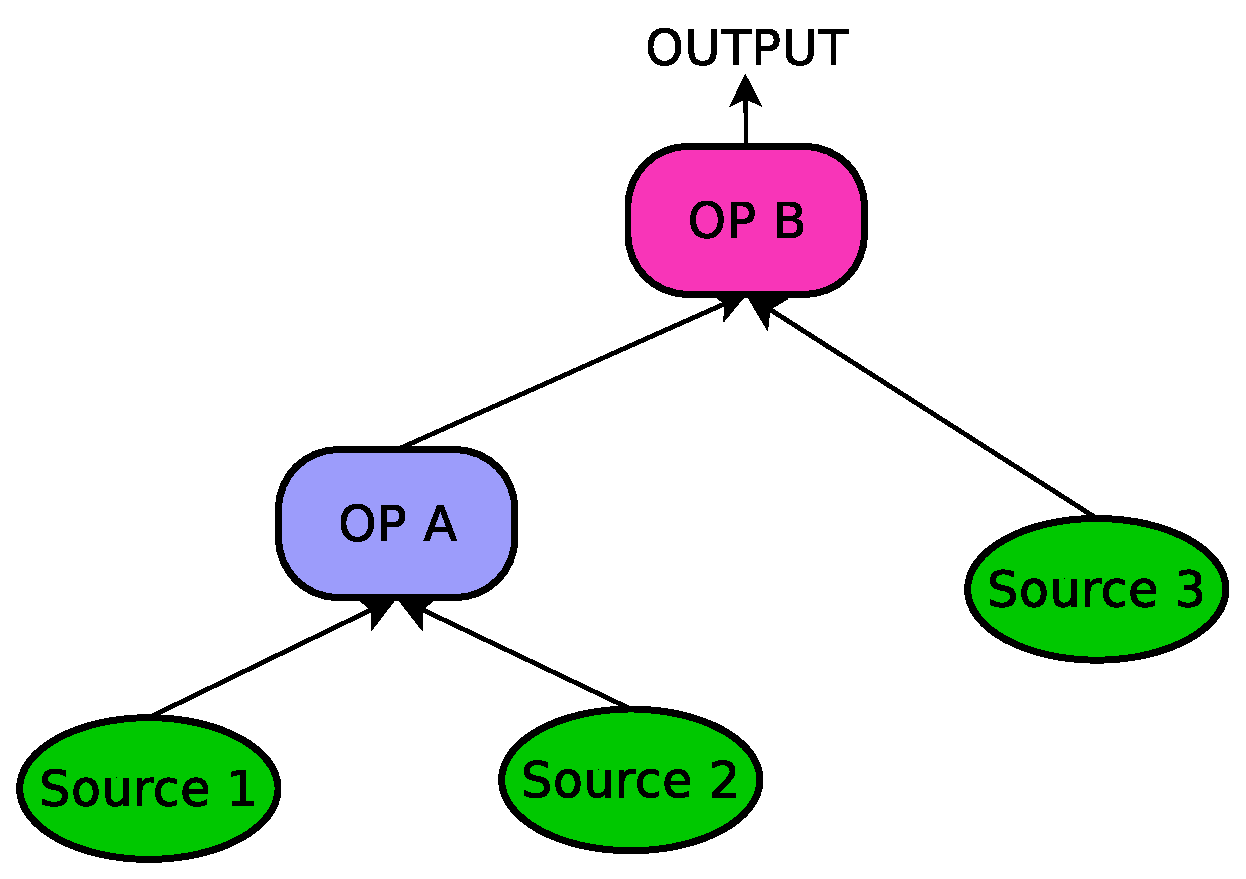
\includegraphics[width=0.55\textwidth]{img/tesi/unbalanced-tree_senza}
	\caption{An unbalanced query tree, showing the different information content of tuples.}
	\label{fig:unbalanced-tree}
\end{figure}

	
	When we consider the importance of an individual tuple within a query, it is important to take into account the
	amount of information that went into its creation. The more information is part of a tuple, the 
	more important it becomes for the computation of the final query result. If the system needs to make a
	decision about which tuples to discard, it has to consider the individual information content of tuples and
	discard the ones with the lowest values first. This is done to reduce the amount of missing information in
	the final query result. 

Let us consider a query whose graph representation resembles an unbalanced tree, as shown in
\mbox{Figure~\ref{fig:unbalanced-tree}}. In this query there are $3$ sources, all producing tuples at the
same rate. The input tuples produced by source 1 and 2 are first combined together by operator A. The
resulting tuples are processed by operator B, together with the tuple produces by source number $3$.
We can assume that the operator B resides on a different machine than operator A and that, due to
overload, it needs to discard one tuple out of the four present in its input buffers. When comparing the
information values of the tuples, the tuples received for the left input stream have an information
content that is twice that of the tuples received on its right input stream. This is because the tuples
on the left contain the information for $2$ sources, while the others carry the
information for a single source. Since the goal of the system is to deliver results with the maximum
amount of source information, the system decides that the tuple to discard should be one of those
received on its right input. \\

\textbf{8. TOTAL INFORMATION CONTENT \\ \textit{The total amount of information contained in a result in
the absence of failure is equal to the number of sources}}

In the absence of failure, every result batch produced by a query contains an amount of information that
is equal to the sum of the individual information values carried by the source tuples.
Considering every source as equal, we can assign a value of $1$ to the complete set of source tuples for
each source that contributed to the calculation of a result batch. If we do so, the final value of a
result batch is equal to the number of sources.

	Let us consider a simple query that calculates an average pollution value every minute from a set of
	$10$ sensors located at different locations in a city. This query produces a result batch of a single tuple,
	which aggregates all the information gathered by the $10$~sensors over a one minute window. Let us
	assume that no failure has happened and that all tuples are correctly processed. Since all sources are
	considered equal, the total amount of information carried by the tuples produced by each source
	over a minute is $1$. When the final result is computed, the total information is equal
	to $10$ (\ie the number of sources).

	When dealing with a system that supports the concurrent execution of multiple queries, it becomes
	important to compare the information values of the different queries. This is needed in
	an overload condition, when trying to achieve \textit{fair shedding}. In fair shedding, the system
	selectively discards tuples to reduce the load of the system so that the final quality values of all
	queries is equalised.
	Therefore, the system must compare the different information content values of tuples. A simple
	way to achieve this is to normalise the information content value by dividing the total
	value of a query result by its number of sources.
	This scales all values in the interval $[0,1]$, making them comparable.\\

\textbf{9. QUERIES ARE DIRECTED ACYCLIC GRAPHS \\ \textit{An operator may have more than one downstream
operator.}}

	A query can be represented as a directed acyclic graph (DAG), in which nodes represent operators and
	arrows the streams flowing through them. This means that, as long as there are no cycles, every operator
	can have multiple downstream operators that receive its output as input. There are two reasons for
	distributing the output of an operator: (1) the query has to compute multiple results; and (2) the
	downstream computation has to be split over multiple machines because it would be too computationally
	intensive for a single one.

The first case deals with queries computing multiple results. These are called \textit{fan-out} queries
and will be further discussed in Section~\ref{sec:fan-out}. They compute multiple results based on common
input information but are logically a single query. The reason for treating a query with multiple results
as a single query is to allow the system to be fair when making shedding decisions under overload.
Let us consider a system with two running queries, submitted by two users. The first user submits a
query with a single terminal operator, while the query submitted by the other user may have $9$.
If the system considered each computed result as a single query, the second user would be allocated 90\%
of the available resources, leaving only 10\% to the first. If the system instead considers the query
submitted by the second user as single computation with $9$ different results, it can evenly discard
tuples among the two queries, leading to a fair allocation of the available computing resources.
Fair shedding will be described in more detail in Section~\ref{sec:fair-shedding}.

	The second reason for the distribution of the output of an operator is when the downstream computation
	is too intensive to be executed by a single machine. In this case, the output is split among several
	processing nodes, each hosting the same set of operators that process a fraction of the output
	tuples.
	The computed results are then collected to produce a single final result. 

	When computing the values of the quality metric, the system needs to take this into account. In
	particular, an operator distributes the total value of information from its input to all its output
	tuples.
	A tuple is assigned a value that is inversely proportional to the number of the output streams of the
	operator. In the first case, when multiple results are calculated, each terminal operator will produce
	tuples with a value equal to the number of sources, divided by the number of results. In this way, the
	cumulative information value for the query is the same as in cases with only a single terminal
	operator.
	The details of this are covered in Section~\ref{sec:sic}.


\section{Types of Queries}
\label{sec:qtypes}

%\mnote{NO numbers in examples, just explanation}

%This section will illustrate how to derive a metric describing the quantity of information captured
%by tuples flowing through a query processing system based on the assumptions stated in
%Section~\ref{sec:assumptions}.

This section introduces a categorisation of different query types, which is
based on the shape of their graphs. When each operator has at most one successor, the query
graph resembles a tree, with input sources as leaves and one output stream as root. Such queries
belong to the \emph{fan-in} type: the number of edges in the graph decreases from sources
to output. 
A query containing operators with more than one successor instead belongs to a \emph{fan-out} type. 
In this case, the query graph can be more complex, with the restriction of being acyclic. Fan-out
queries can have multiple input sources as well as multiple result streams. 
The following sections provides more detail on these two types of queries.

\subsection*{Fan-in Queries}
\label{sec:fan-in}

\begin{figure}[b!]
	\centering
	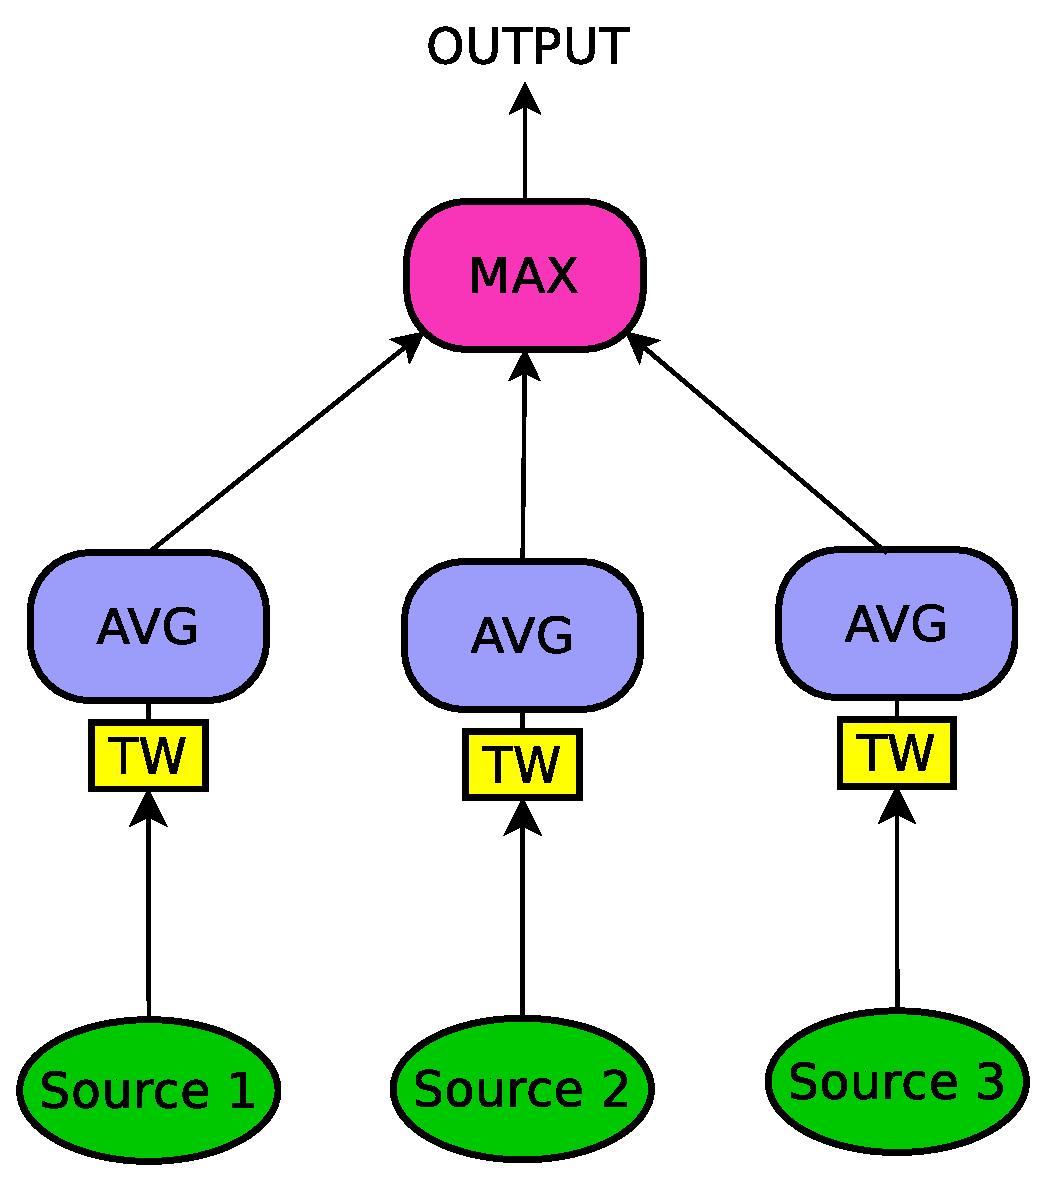
\includegraphics[width=0.35\textwidth]{img/tesi/query_fanin_senza} 
	\caption{An example of a fan-in query. Input values from each source are first averaged over a certain
	time window, and then the maximum is selected.}
	\label{fig:query_fanin}
\end{figure}


In \emph{fan-in} queries, operators have \textit{at most} one successor operator, and the input data from
one or more sources is used to produce a \textit{single result}.
In this category, we find queries computing a single aggregation result.
Such queries have a graph that resembles a tree with many input sources, a series of
processing steps and a single output stream.

\ex Consider the query depicted in Figure~\ref{fig:query_fanin} that calculates
the maximum average value produced by the data sources.
Three sources produce input tuples at different rates. All tuples from a source are first
collected by a time window and then averaged. Finally, the maximum value among the
averages is selected and output. This is a typical fan-in query, in which input tuples from several
sources are collected and processed to produce a single output.

\subsection*{Fan-out Queries} 
\label{sec:fan-out}

\begin{figure}[b!]
	\centering
	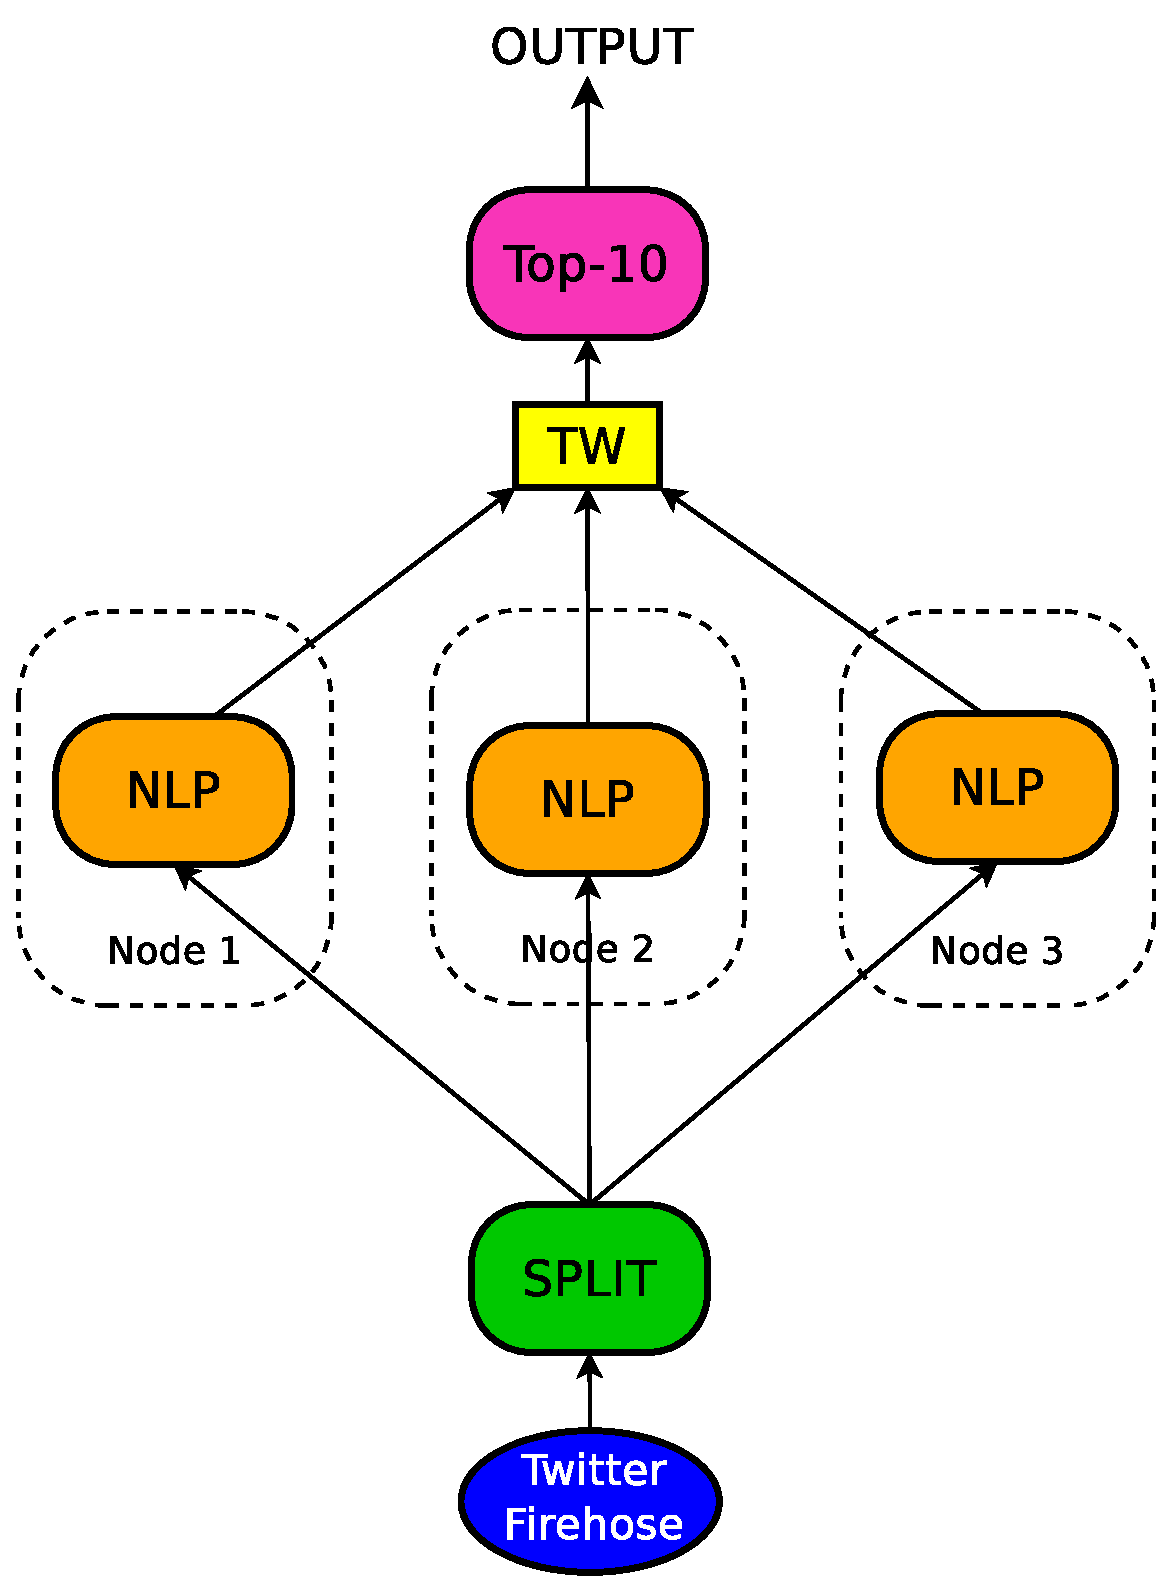
\includegraphics[width=0.45\textwidth]{img/tesi/fan-out_mr_senza} 
	\caption{An example of fan-out query. It processes Twitter data by counting the top-rated messages on a
	certain topic.}
% 	It calculates a value to each tuple based on a natural language processing operator. Due to the heavy
% 	computational cost of these operators, the data is split onto 3 nodes and processed separately. Finally
% 	a max operator determines the message with the highest value.
	\label{fig:fanout_mr}
\end{figure}

The second class of queries that we consider are \textit{fan-out} queries. There one or more operators
send their output to \textit{more than one} downstream operators.
Unlike fan-in queries, whose graph is a tree, a fan-out query
graph can have any configuration, as long as as it does not contain cycles.\\
Fan-out queries can be divided into two possibly overlapping classes: (a) queries with one
result but split computation; and (b) queries with more than one result. Next, we present
examples~for~each~case.

\textbf{Split Computation Queries.} 
Since operators may be computationally too demanding to be hosted on a single processing node, their
computation may have to be split among a number of copies running at different sites. These
copies are composed of the same set of operators but process only a subset of the original data.
Splitting the computation allows the system to spread the processing cost of a set of operators over
multiple nodes and thus overcome an overload condition at a single hosting node. 

\ex Figure~\ref{fig:fanout_mr} shows a query processing Twitter data in
real-time. A stream of Twitter messages can be analysed to calculate the ``top rated'' status updates.
In addition to the message text itself, every message contains information about the location where it
was sent and the author.
\begin{figure}[b!]
	\centering
	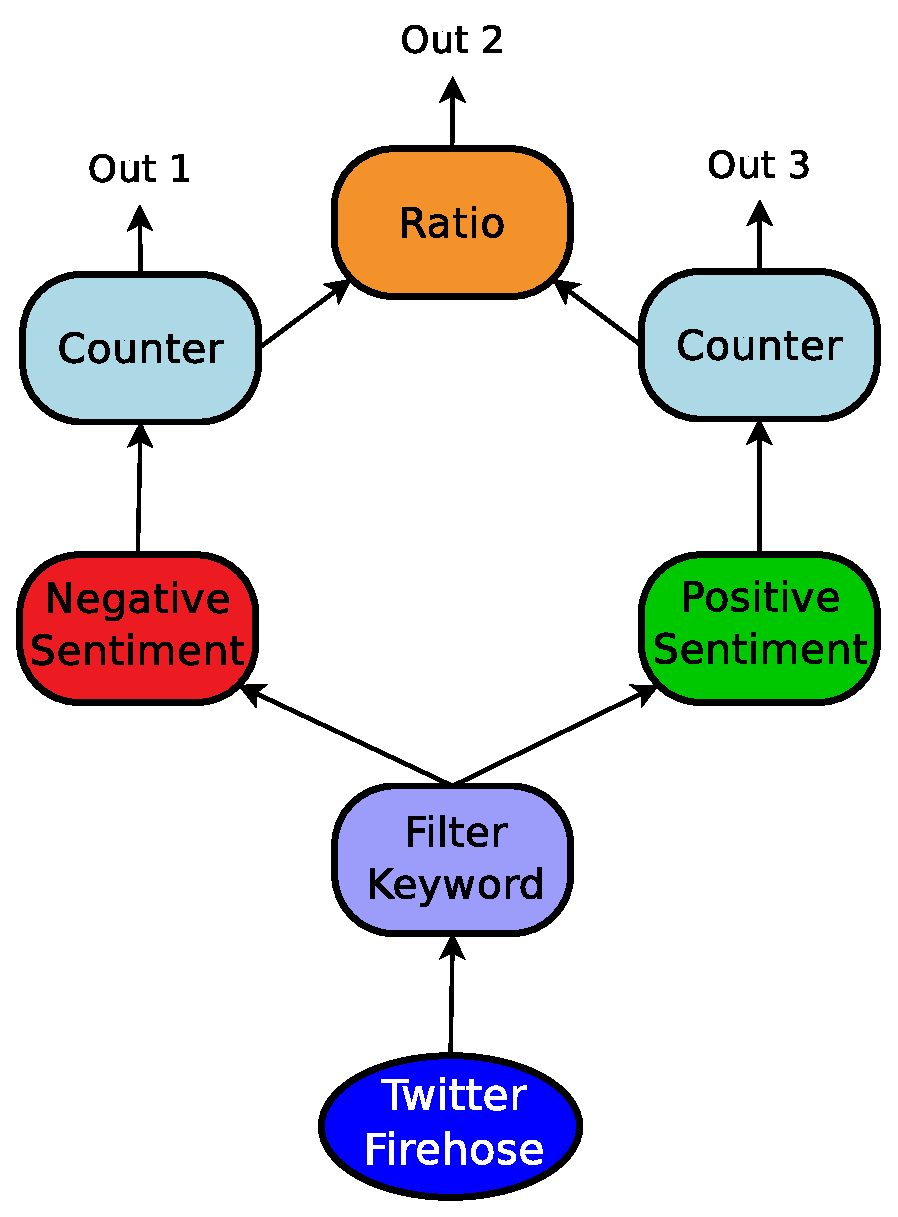
\includegraphics[width=0.4\textwidth]{img/tesi/fan-out_2_senza} 
	\caption{An example of a fan-out query for processing Twitter data. It counts the occurrence of positive
	and negative mentions of a certain keyword and calculates their ratio.}
	\label{fig:query_fanouts}
\end{figure}
A single stream of Twitter messages is split and scattered over three different processing nodes, each
hosting a Natural Language Processing (NLP) operator that calculates some coefficient for each message,
for example, its ``rating''. The output of these NLP operators is collected by a single Top-10
operator preceded by a one minute time-window. The query then outputs then the ten ``top-rated'' Twitter
messages posted every minute. 

\textbf{Multiple Result Queries.} Some queries produce several outputs from the same set of
input data.
These can be seen as multiple single output queries with a partial overlap in their computation. When analysing a
stream of data, a user may be interested in obtaining several different results. Instead of submitting
$N$ queries, they can submit a single fan-out query with multiple end points. Conceptually, this is
simpler than having to design and submit several almost identical queries. It directly exploits the
processing redundancy by reusing a number of streams and operators.


\underline{\textsc{Example}}:~Figure~\ref{fig:query_fanouts} shows a query that calculates the occurrence
of positive and negative statements about particular keywords on Twitter. 
The original stream contains an unsorted stream of messages. First, a filter eliminates all the
messages that do not contain a keyword of interest. After that, the output stream is multiplexed over
two different NLP operators, which forward tweets if they contain
either a positive or a negative mention of a keyword. The resulting streams are sent to a counter
operator, which produces two output streams counting the number of positive and negative references to
a given keyword. The resulting streams from the counter operators are sent to a final operator that
calculates the ratio between them, resulting in an indication of the general feeling about a
keyword. In this query, a single input source is processed to produce~three~different~results.

% The next section will describe the \emph{Source Coverage Ratio} (\sic) quality metric developed in
% the scope of this project, derived following the reasoning of all the model assumptions made in
% Section~\ref{sec:assumptions}.
% In Section~\ref{sec:apps} there will be a further analysis of these sample queries, which will be used as
% running examples of real-world applications of the \sic metric.
 


\section{Source Coverage Ratio}
\label{sec:sic}

%n the previous section I showed how the previously stated assumptions about the quality-centric data
%model can be applied to some generic queries. The goal was to provide an intuitive description about how
%the \sic values are calculated for different query types. In this section I will provide a formal
%definition about \sic calculation.

This section provides the definition of a new quality metric called \emph{Source Coverage Ratio
(\sic)}. A complete set of equations is derived for
its calculation, following the reasoning expressed in the assumptions presented in
Section~\ref{sec:assumptions}. The section finishes with a discussion of the benefits of the \sic metric
when employed by a stream processing system.

\subsection*{Introduction}

Typically a stream processing system does not have global knowledge if all the
available data was processed correctly. 
Therefore, we propose that the impact of failure should be monitored and accounted for. 
In our model, we augment streams with a new metric called \textit{Source Coverage Ratio}
(\sic), which quantifies the amount of information in a tuple, thus recording its
importance for the current query results. The \sic metric is added to streams in the form of metadata,
whose value is calculated by the query operators and is inversely proportional to the level of failure.

A tuple should convey information about the amount of failure experienced during its creation. There
should be a way to indicate if the data carried by a tuple includes all the available
information, making it 100\% accurate, or if some information was lost in the process, thus reducing
its quality. \textit{Source Coverage Ratio} tries to achieve
this goal by measuring the amount of lost information.

The system can use the \sic metric to evaluate the importance of a tuple towards the final query result. 
When the system is overloaded, it has to decide which tuples should
be discarded in order to recover. In this case, \sic values can be used to assess the
individual value of tuples and guide the system to a selection that helps improve the quality of the
results.

% In a single query scenario the system is able to reason about the amount of information carried by
% tuples. By dropping the tuples with the lowest values, it minimises the impact of tuple loss on the query
% results.
% Even in the absence of failure, it is possible that some tuples aggregate more information than others and should
% be preserved with higher priority. In case of failure, the system should discard low valued tuples
% instead.
When only a single query is deployed, the system can minimise the impact of overload by selecting the
tuples to be discarded among those with the lowest \sic values.
When dealing with a system that allows the concurrent execution of multiple queries, \sic values
help discard tuples in a way that affects all queries in the system equally.
We refer to this as \textit{fair shedding}. 
%and it will be further described in Section~\ref{sec:fair-shedding}.

\subsection*{Data Model Formalisation} 
\label{sec:sits}
The purpose of the \sic metric is to capture the amount of information that contributed to the creation
of an output tuple. In the absence of failure, the \emph{perfect value} of the \sic metric is equal to
the number of sources. A reduction from this value is caused by failure during processing. 

Since it is not possible to know in advance which tuples will contribute to the creation of an output
batch of tuples, the final \sic value is not calculated based on individual tuples but instead over a
window of tuples. The amount of information is defined over a time interval so that the final result \sic value
is the sum of the individual \sic values of all tuples produced within the corresponding time window.
Every tuple within the interval is assigned the same value, as for Assumption 5 (Tuple~Equality). All
sources assign the same total \sic value in a time window, as for~Assumption~6~(Source~Equality).

For example, a source producing 100 tuples in a given time interval
assigns a \sic value of 1/100 to each tuple. Another source producing only 20 tuples during the same
time interval assigns individual \sic values of 1/20. The result tuples obtained after processing
would have an aggregated \sic value of 2 without failure.
We refer to the complete set of tuples produced by the sources in a given time interval as the
Source Information Tuple Set.

% \begin{definition} [Source Information Tuple Set]
% %\label{sec:sits}
% The source information tuple set $\mathcal{T}^{S}$ of a result tuple $t_{R}$ is the set of source tuples
% defined by a function $f^{-1}: \mathbb{T}^{R} \rightarrow \mathbb{T}^{S}$ when applied over $t_{R}$, \ie
% $f^{-1}(t_{R})=\mathcal{T}^{S}$.  $\mathbb{T}^{S} = \{ \mathcal{T}^{S}_{s}~|~s \in \mathcal{S}\}$ where
% $\mathcal{T}^{S}_{s}$ denotes the set of source tuples in $\mathcal{T}^{S}$ generated from source $s$.
% \end{definition}
\begin{definition} [Source Information Tuple Set]
%\label{sec:sits}
The source information tuple set $\mathcal{T}^{S}$ of a result tuple $t_{R}$ is the set of source tuples
that contributed to the creation of $t_{R}$ (\ie the set of tuples that were processed by the query
function $f_Q : \mathcal{T}^{S} \rightarrow t_{R}$ to generate $t_{R}$).
\end{definition}
%%\mnote{the definition is taken from the Themis paper but seems a bit too complicated to me.}
In our query model, every result tuple $t_{R}$ is associated with the set of source tuples
$\mathcal{T}^{S}$ that contributed to its creation. We consider a query as a black-box with a \emph{query
function} $f_Q$ that maps source tuples to result tuples. The \textit{source information tuple set} of a
result tuple is the set of all source tuples. 

This concept is central to the definition of the \textit{Source Coverage Ratio} (\sic) quality
centric metric. The intuition behind it is that a result tuple is considered to be perfect when no
information from the sources was lost, meaning that all tuples in its source information tuple set (and
any derived tuples) were processed correctly. If one of the tuples is lost, either due to failure or
deliberate load-shedding, the information contained in the result tuple is not perfect, and its \sic
value is decreased accordingly.

\begin{definition}[Source Coverage Ratio] {
The source information content (\sic) of all result tuples for query $Q$, 
denoted as $\sic_Q$, measures the contribution of all source tuples, belonging to the source
information tuple set $\mathcal{T}^{S}$, in the result tuple set $\mathcal{T}^R$. It is calculated as: 
\begin{align} 
		\sic_Q = \sum_{t_R \in \mathcal{T}^R} t_{R}^{SIC} = \sum_{t_{src} \in \mathcal{T}^{S}}
		t_{src}^{SIC},
\end{align}
where $t_{src}$ are source tuples in $\mathcal{T}^{S}$ used for the calculation of the
result tuples $t_{R}$. In particular, $t_{src}^{SIC}$ shows the contribution of a source tuple from 
source ${src\in\xspace S}$ to the perfect result and is defined by:
\begin{align}
		t^{SIC}_{src} = \frac{1}{|\mathcal{T}_{src}^{\mathcal{S}}||\mathbb{S}|}
\end{align} 
where $|\mathcal{T}_{src}^{\mathcal{S}}|$ is the total number of tuples in the Source Information Tuple
Set of source $src$, and $|\mathbb{S}|$ is the total number of sources in the query. }
\end{definition}
\vspace{-5pt}
Equation~(3.1) states that the total \sic value of all result tuples for a given query, is equal to the
sum of the \sic values of all tuples in the Source Information Tuple Set. 
% It aggregates all the \sic values of all source tuples that contributed to its creation. 
Since a query can have multiple terminal operators, each potentially producing more than one result
tuple at the time, we consider the \emph{sum} of all the result tuples produced by all terminal
operators.
If all tuples are correctly processed, the
resulting \sic value is 1. A lower value indicates that some information loss happened
during the query execution.

Equation~(3.2) describes how source tuples are assigned their individual \sic values. First, a value of 1
is assigned to the totality of tuples produced by a source in its Source Tuple Information Set. This
means that all sources are considered to contribute equally to the final result, regardless of the amount
of tuples that they produce during an interval.
Since every tuple in this set is considered to contain the same amount of information, this value is
divided by the number of tuples produced by the source during a time interval.
Thus, the \sic value of an individual source tuple $t_{src}$ is inversely proportional to the number of
tuples in $|\mathcal{T}_{src}^{S}|$. Furthermore, it is necessary to normalise by the number of sources
$|\mathbb{S}|$ connected to a query, dividing the initial \sic values by the number of sources.
In this way, all resulting \sic values are in the interval $[0,1]$, which makes it possible to compare
the quality of different queries.
\vspace{-10pt}
\subsubsection*{\sic Propagation from Source to Result Tuples}
\vspace{-5pt}
Up to now, we considered queries as black-boxes and discussed only the relation of \sic values between
the source and result tuples. In order for the formal description to be complete, it is important to
understand how intermediate \sic values are calculated at individual operators and how these propagate
within the system.

Source tuples from $\mathcal{T}^{S}$ are processed by the query operators in the set $\mathcal{O}$, which
produce new derived tuples. These tuples flow to the next downstream operator until they reach a terminal
operator that outputs result tuples.
More formally, for a given intermediate derived tuple $t_{out}^{o}$ and for an operator $o \in
\mathcal{O}$, we define $\mathcal{T}_{in}^{o}$ to be the set of all input tuples to an operator $o$ required for the
generation of $t_{out}^o$.
Similarly, $\mathcal{T}_{out}^{o}$ denotes the set of derived tuples produced by operator $o$ after the
processing of $\mathcal{T}_{in}^{o}$.

The \sic value of a derived tuple $t$, processed by operator $o$, (\ie $t \in \mathcal{T}_{out}^{o}$) is:
% \begin{align} t_{SIC} = \frac{\displaystyle\sum_{t \in
% \mathcal{T}_{in}^{o}}{t_{SIC}}}{|\mathcal{T}_{out}^{o}|}.
% \end{align}
\begin{align} 
	t^{SIC}_{out} = \frac{1}{|\mathcal{T}_{out}^{o}|} \cdot \displaystyle\sum_{t_{in} \in
	\mathcal{T}_{in}^{o}}{t^{SIC}_{in}}
\end{align}
This means that the set of derived tuples produced by an operator contains all the information from the
input tuples that the operator processed. This information is considered to be distributed equally over
all the output tuples: the total value is divided by the number of output tuples.

The way that the \sic values are calculated is recursive: it is the same if a
single operator or a complete query, seen as a complex black-box of operators, are considered. The sum of
the information for the input is always propagated to the output tuples and equally divided among them. 
\vspace{-10pt}
\subsubsection*{Relation of \sic to Query Processing Quality} 
The \sic values of result tuples lie in the $[0,1]$ interval: \\
(a) A value equal to $1$ indicates that the complete set of $\mathcal{T}^{S}$ tuples was
used during processing and that the result is perfect. \\
(b) A value of $0$ indicates that all source tuples from $\mathcal{T}^{S}$
were discarded or lost during processing. \\  
(c) A value between $(0,1)$ indicates a degraded result, meaning that only a subset of the tuples
contained in the Source Tuple Information Set was used for computation. A small value means a
large information loss, while a value close to 1 indicates an almost perfect result. 
\subsubsection*{Model Benefits}

\textbf{Query Performance.} Even though \sic values provide a good estimate of the quality of the
processing, it should be noted that their value is not linked directly to the absolute error of the query
results. In general it is not possible to compute error bars on the delivered results based on this
metric.
\sic values are an indication to the user about the amount of failure that occurred during the generation
of a query result. It is then up to the user to decide if the delivered answer should be considered valid
or should be discarded. 

Nevertheless \sic values are a good indication about the quality of the results. The
knowledge of the query semantics may allow a user to correlate \sic values with an absolute result error. 
The simpler the query semantic, the easier it is to establish such a correlation. 

\textbf{Completeness of Results.} Using \sic values, it is possible to compare the results of the same
query at different times to evaluate the quality of the results in terms of information
completeness. A result tuple $t^R_1$ delivered a time $t_1$, compared to another result tuple $t^R_2$
delivered at time $t_2$, contains more information if and only if $t^{SIC}_1 > t^{SIC}_2$.

A user can monitor the status of a computation by observing the changes in \sic values of a
query at different times. A decrease in \sic values means that more information was
discarded, and there may be a need to act upon it. Reasons for a sudden reduction may be:\\
(1) the failure of one or more processing nodes, requiring the migration of some operators and
recovery of the failed infrastructure; or\\
(2) a sharp increase in input rates, requiring the increase of processing resources to maintain \sic
values within acceptable bounds.

\textbf{Fair Resource Allocation.} Using \sic values, it is possible to compare the performance
achieved by different queries running concurrently on a shared processing platform. A fair system would
try to equalise the quality of processing of running queries, allocating resources in such a way as to
provide results with similar \sic values for all queries.

When the system experiences \emph{overload} and needs to discard a certain number of tuples, it can use
the \sic values to determine which tuples to drop and which tuples to preserve. This process is achieved
through \emph{fair shedding} and will be further explored in Section~\ref{sec:fair-shedding}.
\vspace{-10pt}

\section{Use Cases for Source Coverage Ratio}
\label{sec:apps}

This section returns to the sample queries of Section~\ref{sec:qtypes} to illustrate the
calculation of \sic.
\vspace{-10pt}
\subsection*{Fan-in Queries}

In Figure~\ref{fig:query_fanin2}, the final \sic value obtained by the depicted query is $3$, which is
equal to the number of input sources.
This follows from Assumption $8$ (Total Information Content). To simplify the exposition, we show
absolute values (\ie not scaled to the $[0,1]$ interval for comparison). It is also a perfect value (\ie
there was no loss of information during processing). In the case of failure, its value
would be reduced by the amount of information contained in the lost tuples.

According to Assumption $4$ (Source Equality), all sources contribute equally to the creation of the
final result.
Assumption $5$ (Tuple Equality) states that all tuples from a source in the \textit{source
information tuple set} contain the same amount of information. 

Figure~\ref{fig:query_fanin2} shows that
each source assigns a total value of 1 to the tuples belonging to the same source information tuple set window, and
that the individual \sic values are different according to the number of tuples contained in it. In this
example, the first source produces only 2 tuples and thus the individual \sic value is $1/2$; the second
source produces 4 tuples with an individual value of $1/4$; and the third 3 tuples, each with a value of
$1/3$.
\begin{figure}[h] \centering \includegraphics[width=0.35\textwidth]{img/tesi/query_fanin} \caption{An example of fan-in query. Input values for each source are first averaged over a certain time window, and
then the maximum value is selected. Source Coverage Ratio values are shown for each tuple.}
\label{fig:query_fanin2}
\end{figure}

The \textit{average} operator takes in input a batch of tuples of size 2, 3 and 4, respectively, and
outputs a single tuple. Assumption 6 (Conservation of Information) requires that the amount of
information going into an operator is equal to the amount in the output. Therefore, the newly generated
tuples are all assigned a \sic value of 1, which is the sum of the individual \sic values of the input
tuples.

The final \textit{max} operator inputs 3 tuples, each with a \sic value of 1, and outputs a single
tuple with a \sic value of 3. Even though the processing semantics of the max and average operators are
different, the calculation of \sic values remains the same, as required by Assumption 3 (A Generic
Metric).
The final tuple contains the total amount of information carried by all the initial input tuples. 

Let us consider what would happen to the final \sic value in case of the loss of a tuple, for example, a
source tuple produced by Source 2. In this case, the amount of information in the tuple generated by the
central average operator would be $3/4$ instead of $1$. The loss of information (\ie to the amount
of $1/4$) would then be propagated to the final tuple, which would have a \sic value of $11/4$ instead of
$3$.
Since the calculation of the \sic values is additive, the amount of information missing, compared to
the maximum value, is equal to the sum of the \sic values of the individual tuples that
were lost during processing.

\subsection*{Fan-out Queries}

\textbf{Split Computation Queries.} Figure~\ref{fig:fanout_mr} shows a query that processes 300 messages
during a time window. Each message is analysed by a Natural Language Processing (NLP) operator that calculates a
coefficient based on its text. Finally, a max operator outputs the message with the highest coefficient. 

We assume that the NLP operator is computationally intensive and would overload a single node at the
current rate. Therefore the computation is split across 3 different nodes. Each node processes 1/3 of
the messages, and all nodes manage to process all the messages without the need to discard data.
The \textit{split} operator creates a partition of the original stream without data
duplication, which means that the tuples that it outputs still have the same \sic value as the ones in
the input.

This follows from Assumption 9 (Queries are DAGs). In this query, the split operators receive as input
300 tuples. Each with a \sic value of 1/300.  The operator outputs 100 tuples on each output stream,
again with an individual \sic value of 1/300. Each stream is sent to a different processing node where a
NLP operator assigns a coefficient to each message. These operators output the same number of tuples
that they receive as input, thus producing 100 tuples each with an individual \sic value of 1/300.
Finally, all the tuples are processed by a Top-10 operator, which outputs the 10 tuples with the
highest coefficients. Each output tuple has a \sic value of 1/10, for a total final \sic value~of~1.

\begin{figure}[t!]
	\centering 
	\includegraphics[width=0.5\textwidth]{img/tesi/fan-out_mr} 
	\caption{An example of a fan-out query processing Twitter data. 
	The Source Coverage Ratio values are shown for each tuple.}
	\label{fig:fanout_mr}
\end{figure}
\vspace{15pt}
\textbf{Multiple Results Queries.} Figure~\ref{fig:query_fanout} shows a query calculating the
occurrences of positive and negative mentions of a given keyword. 
This query computes 3 different results: the number of messages with a positive mention of a keyword,
the number of with a negative one and their ratio.
The original stream comes from the Twitter platform and contains an unsorted stream of messages. In our
example, during a time window, there are 3 messages with individual \sic values of 1/3. A filter
operator selects only those messages that contain a given keyword, in our example outputting 2
tuples.
At this point, the output of the filter operator is multiplexed over two different operators,
one that filters only messages with positive references to the keyword and one filtering negative
references.
\clearpage
\begin{figure}[b!]
	\centering
	\includegraphics[width=0.45\textwidth]{img/tesi/fan-out_2} 
	\caption{An example of fan-out query processing Twitter data. It counts the occurrences of positive and
	negative mentions of a given keyword. The numbers shown on tuples are their individual \sic values.}
	\label{fig:query_fanout}
\end{figure}

Assumption 9 (Queries are DAGs) requires that, when such a duplication of the
output occurs, the total \sic value must be distributed over all output tuples. This is also in
accordance with Assumption 6 (Information Conservation) because the amount of information in the input is
equal to the amount in the output.
Each output stream of the \emph{keyword filter} operator contains an identical set of 2
tuples, each with an individual \sic value of 1/4.
The positive and negative filters each output a single tuple with a \sic value of 1/2. 

These output tuples propagate to \emph{counter} operators. These operators produce 2 output
streams: one that is terminal and is delivered as a result and another that feeds into a \emph{ratio}
operator.
Again the output of the counter operators is multiplexed and thus the individual \sic values of
the produced tuples are scaled accordingly. In our example, each counter produces 2 identical batches of
1 tuple with a \sic value of 1/4. The ratio operator outputs the third result of the query, producing a
single tuple with a \sic value of 1/2.
The result tuples have different \sic values: 1/4 for the
ones produced by the counter operators and 1/2 the ones produced by the ratio operator. If we sum
these together, we obtain a total \sic value of 1 for the query, which indicates that
no failure occurred during processing. 




\section{Summary}

This chapter presented a data model for stream processing systems that takes the quality of the
processing into account.
First, we defined basic entities, such as tuples, streams and queries. The need for handling and
quantifying failure led to the introduction of a quality metric called the Source Coverage Ratio
(\sic). The definition of this metric followed the reasoning outlined in a set of assumptions and
considerations, making it applicable to a generic stream processing system supporting any kind of
operators.
After that, there was an introduction of the different classes of queries, namely fan-in and fan-out
queries.
This led to the definition of the \sic metric with a set of equations for its calculation. A few
real-world queries were then used to show how the metric can be used to keep track
of the amount of failure that occurred during processing.
The next chapter describes the design of a stream processing prototype system that implements the
quality-aware query model, thus exploiting the \sic quality metric in practic.


	
% \begin{figure}
% 	\centering
% 	\includegraphics[width=0.9\textwidth]{img/tesi/query_topk} 
% 	\caption{An example of query calculating the currently least loaded nodes with at least 1 Gb of free
% 	memory on PlanetLab.}
% 	\label{fig:query_topk}
% \end{figure}


%\input{data_model/ic}
%\emph{3 weeks. This chapter needs a lot of work since we still have to come up with a revised model that can unify the two scenarios. Before coming to London I am going to think about this so that we can together about it in the first meeting. Hopefully this part will be defined by the end of my staying.}

